\documentclass[tikz,border=8pt]{standalone}
\usepackage{pgfplots}
\usepgfplotslibrary{groupplots}
\pgfplotsset{compat=1.18}
\begin{document}
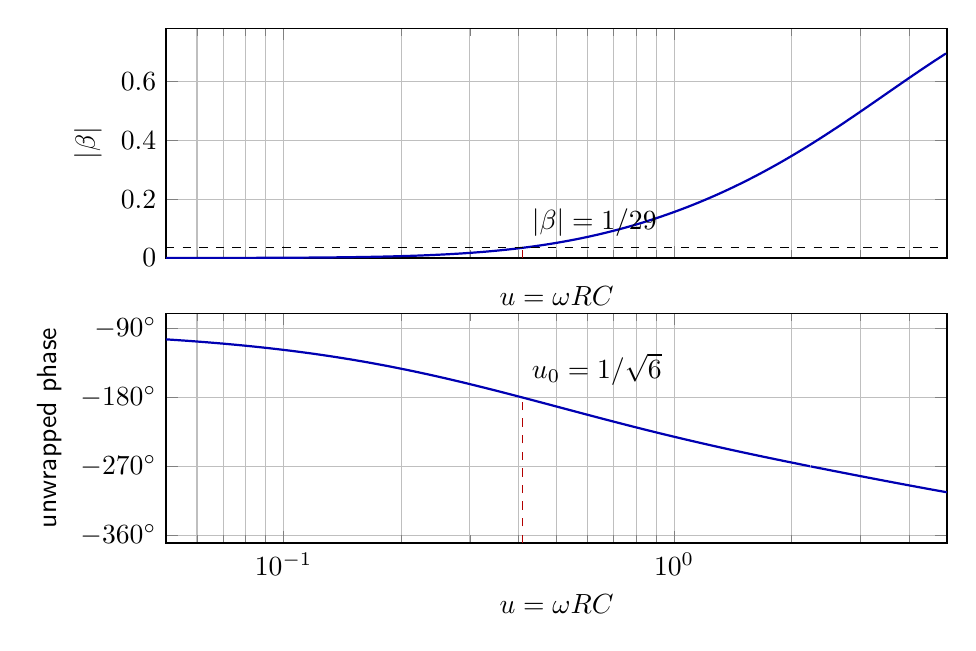
\begin{tikzpicture}[font=\sffamily]
\begin{groupplot}[group style={group size=1 by 2,vertical sep=7mm},width=11.5cm,height=4.5cm,xmode=log,xmin=.05,xmax=5,grid=both,xlabel={$u=\omega RC$}]
\nextgroupplot[ylabel={$|\beta|$},ymin=0,ymax=.78,xticklabels=\empty]
\addplot[blue!70!black,thick,domain=.05:5,samples=500] {x^3/sqrt((1-6*x^2)^2+(5*x-x^3)^2)};
\addplot[black,dashed] coordinates {(.05,1/29) (5,1/29)};
\draw[red!70!black,dashed] (axis cs:.408248,0)--(axis cs:.408248,.0344828);
\node[above right] at (axis cs:.408248,.04) {$|\beta|=1/29$};
\nextgroupplot[ylabel={unwrapped phase},ymin=-370,ymax=-70,ytick={-90,-180,-270,-360},yticklabels={$-90^\circ$,$-180^\circ$,$-270^\circ$,$-360^\circ$}]
\addplot[blue!70!black,thick,domain=.05:2.236,samples=350] {-90-atan2(5*x-x^3,1-6*x^2)};
\addplot[blue!70!black,thick,domain=2.237:5,samples=160] {-450-atan2(5*x-x^3,1-6*x^2)};
\draw[red!70!black,dashed] (axis cs:.408248,-370)--(axis cs:.408248,-180);
\node[above right] at (axis cs:.408248,-177) {$u_0=1/\sqrt6$};
\end{groupplot}
\end{tikzpicture}
\end{document}
